%%%%%%%%%%%%%%%
%
% $Autor: Wings $
% $Datum: 2020-01-29 07:55:27Z $
% $Pfad: General/SensorAPDS9960.tex
% $Version: 1785 $
%
%
%%%%%%%%%%%%%%%

\chapter{\textcolor{red}{Martens: Sensormodul APDS9960 for Gesture, Proximity, and Color Detection}}



\section{Sensormodul APDS-9960}

Das Modul APDS-9960 ist ein Produkt der Firma Broadcom, ehemals Avago Technologies, mit Sitz in San José, Kalifornien. Es handelt sich hierbei um einen Sensor für die Gesten-, Abstands-, Umgebungslicht- und Farberkennung \cite{Avago:2015}.  Ein sehr bekannter Anwendungsfall für diesen Sensor ist das automatische Ausschalten des Smartphone-Displays beim Anlegen des Smartphones an ein Ohr. Hier erkennt der Sensor mithilfe des Abstandssensors, dass etwas auf oder am Bildschirm anliegt. Hier findet die detaillierte Betrachtung des Sensors in Bezug auf die Anwendung als Farbsensor statt. 

Bei der Farberkennung misst der Sensor die Intensität der roten, grünen und blauen Farbe und gibt für jeden Farbkanal einen 16-Bit-Wert zurück. Insgesamt ergibt sich somit auf einen Wertebereich von 0 bis 65535 für eine Farbe. 

Zum Nachvollziehen eines Farbsensors kann das menschliche Auge betrachtet werden. Der Mensch nimmt seine Umwelt optisch über Rezeptoren, die Stäbchen und Zapfen, wahr. Hierbei sind ``die Stäbchen für den Hell-Dunkel-Kontrast und die Zapfen für die Farberkennung'' zuständig \cite{Hering:2017}. Entscheidend sind die Primärfarben Rot, Grün und Blau. Jede weitere Farbe kann aus diesen drei Farben gemischt werden. Aus Farbtabellen lassen sich dann die einzelnen Werte für R-G-B, für die verschiedenen Farben wie beispielsweise Orange, Violett oder Türkis, entnehmen. 

Um den APDS-9960 betreiben zu können wird eine Spannung von 3,0 V empfohlen. Ferner sollte der Sensor zwischen -30$^\circ$C und 85$^\circ$C betrieben werden.

\Mynote{cite books, applications, board}


\section{General}

General description: Farberkennung

\Mynote{cite books}

\section{Specific Sensor}

\Mynote{cite board}

\section{Specification}

\begin{itemize}
    \item cite data sheet
    \item Circuit Diagram
\end{itemize}


\section{Bibliothek}

Im Fall des Sensor APDS-9960 bietet Arduino eine Bilbiothek \FILE{Arduino\_APDS9960} für das Aufrufen der Farberkennung, des Abstandes oder der Gestenerkennung.

Die Bibliothek für den Sensor ist  die  Bibliothek \FILE{Arduino\_APDS9960}. Diese erlaubt es, Gesten, Farben, Lichtintensität und Abstände mit dem Sensor zu messen. Dabei findet die Kommunikation zwischen dem Chip des Arduino Nano 33 BLE Sense Lite und dem Modul APDS-9960  über eine interne I\textsuperscript{2}C-Schnittstelle statt \cite{Avago:2015}.

Die Bibliothek wird durch den Befehl \PYTHON{\#include <Arduino\_APDS9960.h>} eingebunden.


Die aktuelle Version ist 1.0.4 (Stand: 17.04.2024).






\subsection{Description}

Die Bibliothek \FILE{Arduino\_APDS9960} stellt eine Klasse \PYTHON{APDS} zur Verfügung. Mit Hilfe dieser Klasse können auf alle Funktionen zugegriffen werden. \cite{Avago:2015}.

The sensor APDS-9960 has the functionality of proximity distance measure, RGB color detection, and Gesture detection too. Go to example, check the library APDS-9960 and upload the complete program as shown in the figure \ref{fig:1}. Full example includes the RGB color detection code, gesture detection code, and also proximity distance measure code.


\begin{center}
    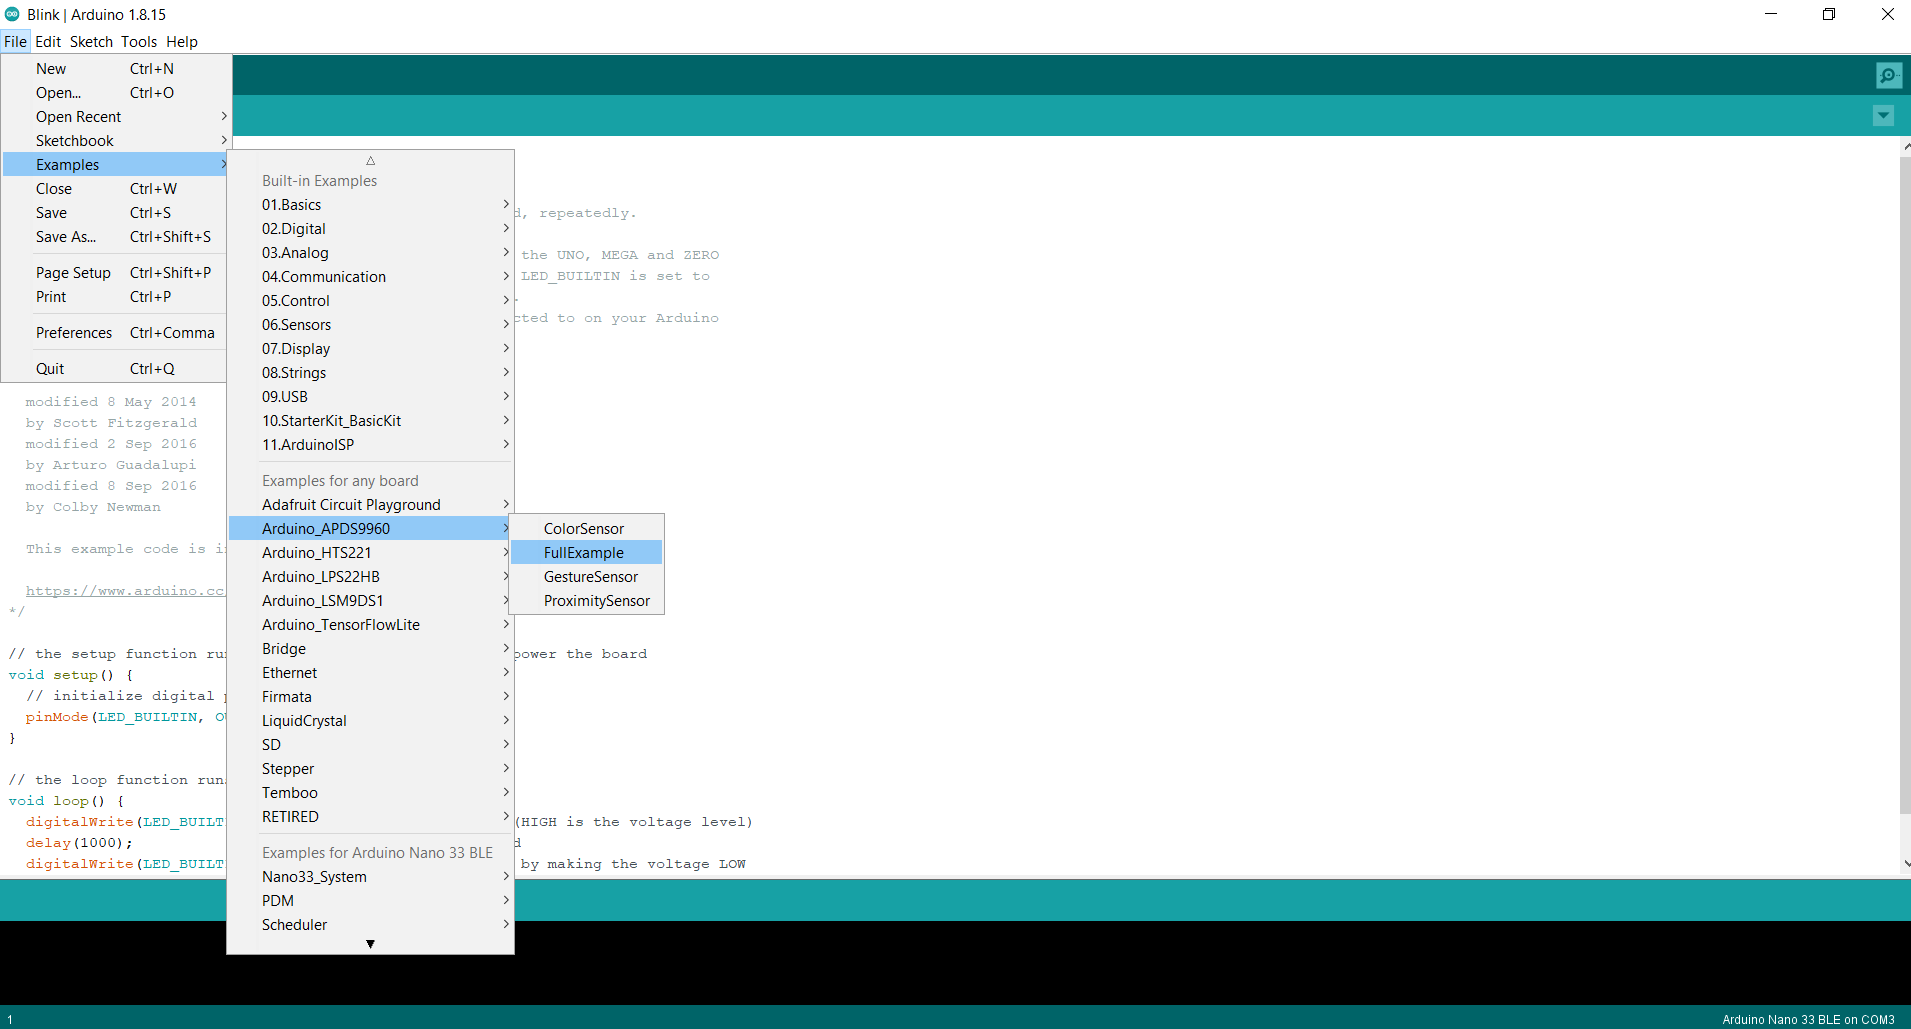
\includegraphics[width=\textwidth]{Nano33BLESense/APDS}
    \captionof{figure}{APDS-9960 Gesture, Proximity, Color Sensor}
    \label{fig:1}
\end{center}








\subsection{Installation}

\menu[,]{Tools,Manage libraries ...}

\begin{center}
  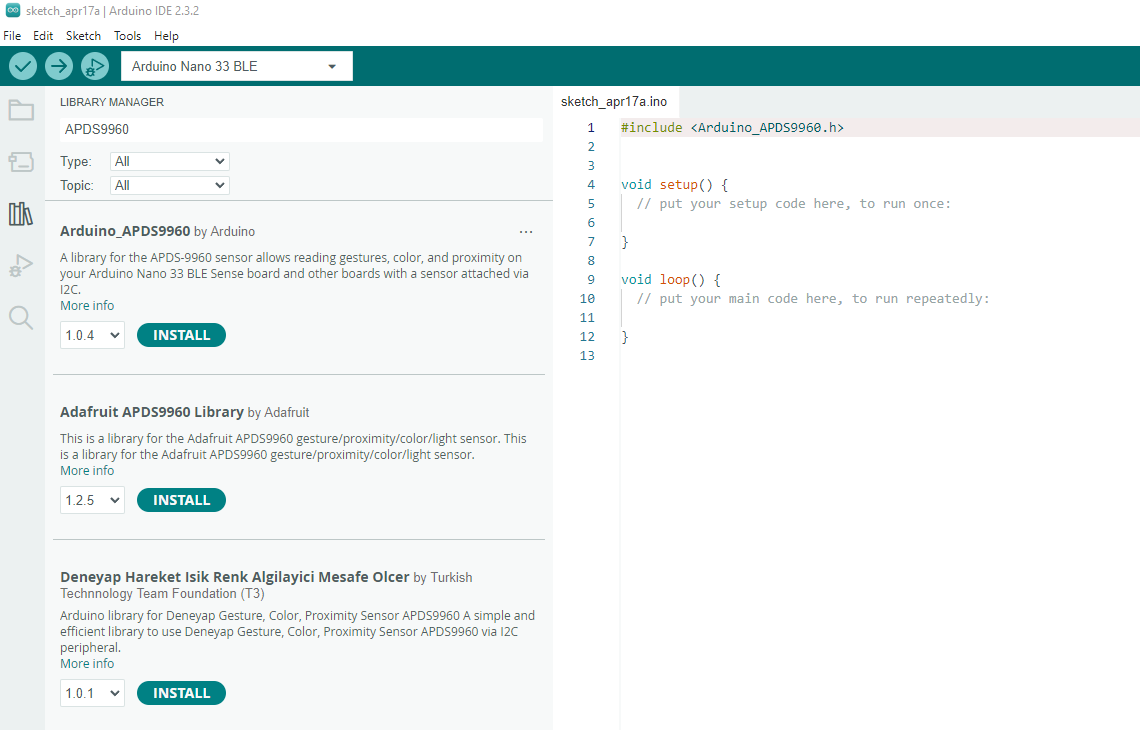
\includegraphics[width=\textwidth]{Arduino/APDS9960/APDS9960Install}
  \captionof{figure}{APDS-9960 Gesture, Proximity, Color Sensor}
  \label{APDS9960Install}
\end{center}

\begin{center}
    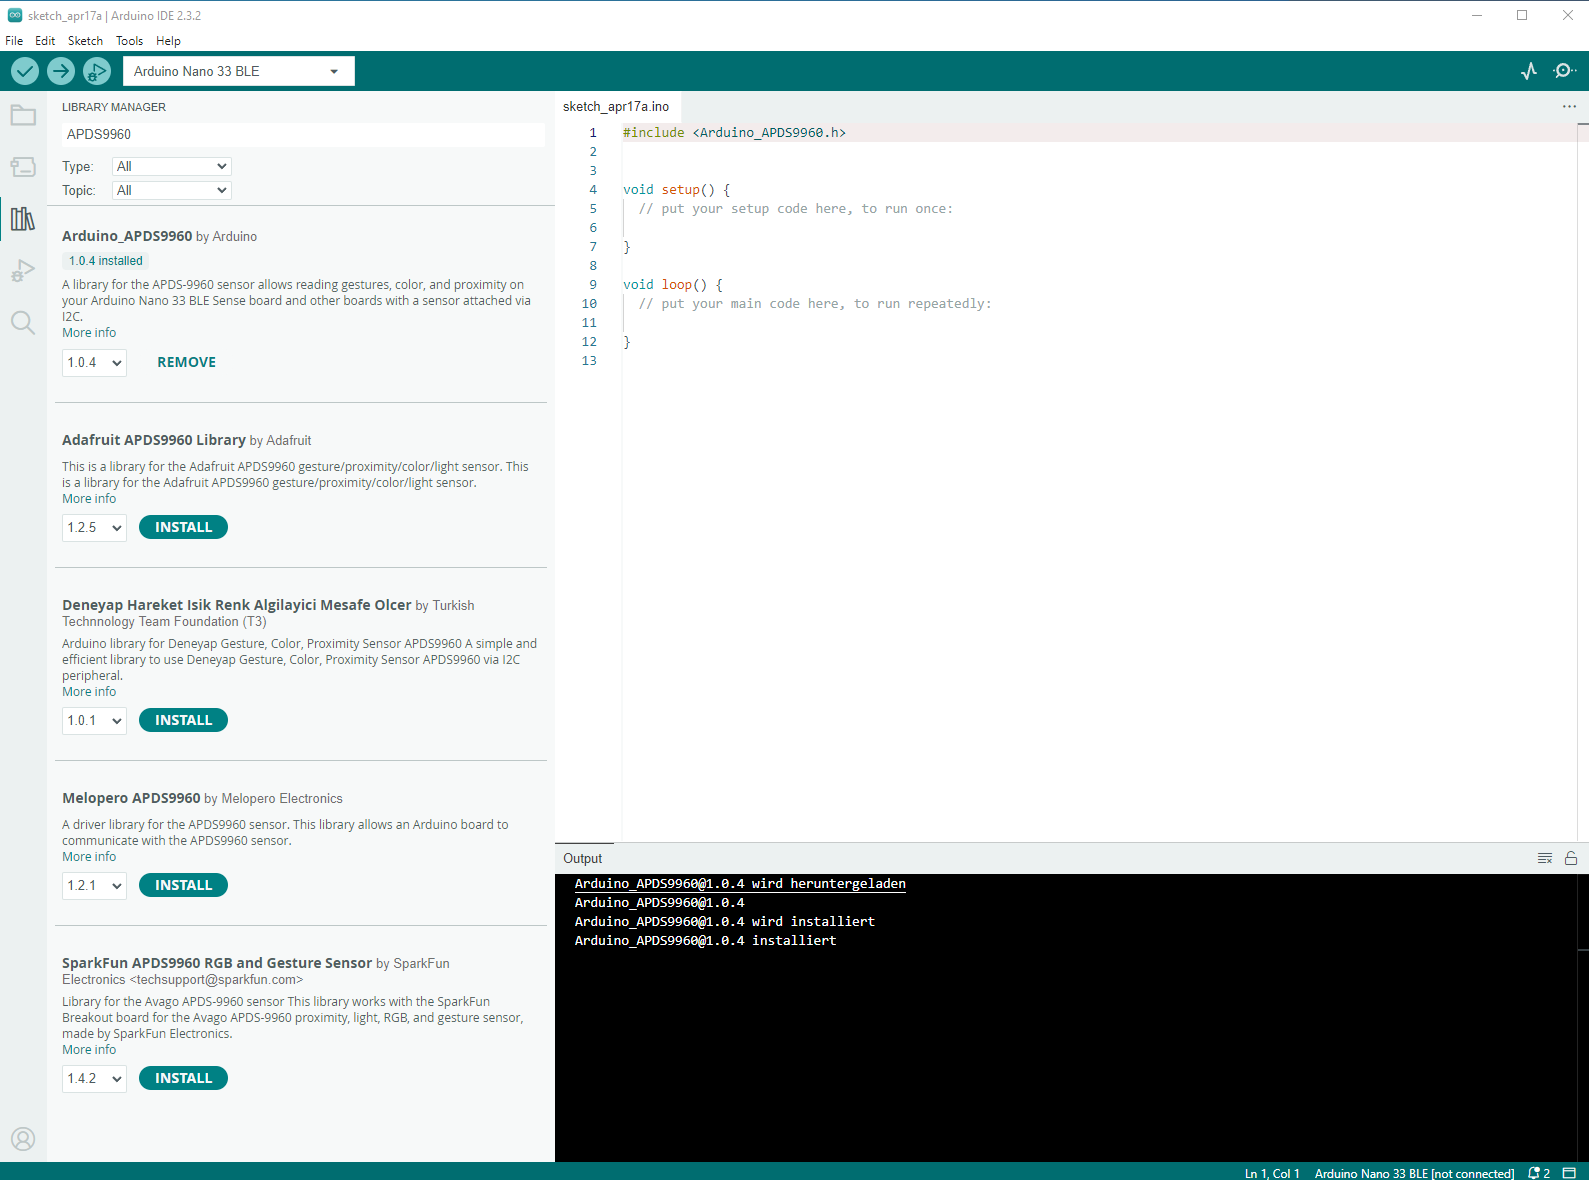
\includegraphics[width=\textwidth]{Arduino/APDS9960/APDS9960Installed}
    \captionof{figure}{APDS-9960 Gesture, Proximity, Color Sensor}
    \label{APDS9960Installed}
\end{center}


\subsection{Functions}

\begin{itemize}
  \item \PYTHON{begin()}: Die Methode \PYTHON{begin()} aktiviert und initialisiert den Sensor APDS9960. Die Methode wird in der Initialisierung \PYTHON{setup\{\}} aufgerufen.
  
        \medskip
        
        \begin{itemize}
          \item Rückgabewert \PYTHON{TRUE}: Die Initialisierung ist erfolgreich gewesen.
          \item Rückgabewert \PYTHON{FALSE}: Die Initialisierung war nicht erfolgreich.
        \end{itemize}
  
  \item \PYTHON{end()}: Die Methode \PYTHON{end()} deaktiviert  den Sensor APDS9960.
      
    
  \item \PYTHON{colorAvailable()}: Die Methode überprüft, ob eine Farbinformation abgerufen werden kann.

        \medskip

        \begin{itemize}
          \item Rückgabewert \PYTHON{TRUE}: Es liegt eine Farbinformation vor.
          \item Rückgabewert \PYTHON{FALSE}: Es liegt keine Farbinformation vor.
        \end{itemize}

  \item \PYTHON{readColor(...)}: Die Methode ermittelt die Farbwerte des Sensors.

        Die Methode bestimmt etnweder nur die Farbwerte oder die Farbwerte und die Intensität des Umgebungslichts.

        \medskip

        Aufruf zur Bestimmung der Farbwerte:

        \PYTHON{int r,g,b;}

        \PYTHON{APDS.readColor(r, g, b); }

        \medskip

        Die Variable \PYTHON{r}, \PYTHON{g} und \PYTHON{b}  enthalten nach dem Aufruf die aktualisierten Farbwerte. Der Wertebreich ist $0, 1, 2, \ldots, 255$.

        \medskip

        Aufruf zur Bestimmung der Farbwerte und der Intensität des Umgebungslichts:

        \PYTHON{int r,g,b,a;} 

        \PYTHON{APDS.readColor(r, g, b); }

        \medskip

        Die Variable \PYTHON{r}, \PYTHON{g} und \PYTHON{b}  enthalten nach dem Aufruf die aktualisierten Farbwerte. Die Variable enthält die Intensität des Umgebungslichts. Der Wertebreich ist $0, 1, 2, \ldots, 255$.
  
  \item \PYTHON{proximityAvailable()}: Die Methode überprüft, ob eine Abstandsinformation abgerufen werden kann.

        \medskip

        \begin{itemize}
          \item Rückgabewert \PYTHON{TRUE}: Es liegt eine Abstandsinformation vor.
          \item Rückgabewert \PYTHON{FALSE}: Es liegt keine Abstandsinformation vor.
       \end{itemize}

  \item \PYTHON{readProximity()}: Die Abstandsinformation wird ausgelesen.
  
        \medskip

        \begin{itemize}
          \item Rückgabewert \PYTHON{int proximity = APDS.int proximity()}: Der Abstand wird als Rückgabewert zurückgegeben.
          \item Rückgabewert \PYTHON{-1}: Ein Abstand konnte nicht ermittelt werden.
       \end{itemize}
   
  \item \PYTHON{gestureAvailable()}: Die Methode überprüft, ob eine Geste erkannt wurde.

        \medskip

        \begin{itemize}
          \item Rückgabewert \PYTHON{TRUE}: Es liegt eine Geste vor.
          \item Rückgabewert \PYTHON{FALSE}: Es liegt keine Geste vor.
       \end{itemize}

  \item \PYTHON{setGestureSensitivity()}: Die Gestenerkennung hängt unter anderem von den Lichtverhältnisse, der Geschwindigkeit und des Abstands der Bewegung ab. Hier kann die Empfindlichkeit der Erkennung eingestellt werden. Ein höherer Wert erkennt mehr Gesten, aber die Fehlerwahrscheinlichkeit für das Erkennung einer Geste, die keine gewesen ist, ist höher. Bei einem niedrigen Wert werden vollzogene Gesten eher nicht erkannt. 
  
        Der Wertebereich ist \PYTHON{1} bis \PYTHON{100}.
  
        Der voreingestellte Wert ist \PYTHON{80}.
        
  \item \PYTHON{readGesture()}: Falls eine erkannte Geste vorliegt, kann diese mit der Methode \PYTHON{readGesture()} abgerufen werden. Dabei stehen 5 mögliche Rückgabewerte zur Verfügung:
  
       \begin{itemize}
         \item \PYTHON{GESTURE\_UP}: Eine Bewegung von unten nach oben wurde erkannt.
         \item \PYTHON{GESTURE\_DOWN}: Eine Bewegung von oben nach unten wurde erkannt.
         \item \PYTHON{GESTURE\_LEFT}: Eine Bewegung von rechts nach links wurde erkannt.
         \item \PYTHON{GESTURE\_RIGHT}: Eine Bewegung von links nach rechts wurde erkannt.
         \item \PYTHON{GESTURE\_NONE}: Keine der vorherigen Bewegungen wurde erkannt. 
      \end{itemize}
      
  \item \PYTHON{setInterruptPin()}: Die Messung wird durch das Setzen eines Eingangs ausgelöst. Dieses Eingang wird in der Regel automatisch erkannt. Mit dieser Funktion kann die Nummer des Pins gesetzt werden.
  
        Falls der Wert \PYTHON{-1} verwendet wird, dann ist kein Pin verbunden.
  
        Falls der Wert \PYTHON{0} oder höher ist, so wird dieser Pin verwendet.
  
        Der Standardwert hängt vom Board ab.
  
  \item \PYTHON{setLEDBoost(...)}: In dem Sensor ist eine Infrarot-LED integriert. Die LED kann kurzfristig mehr Leistung um heller zu sein. Es kann bis zum 3-fachen der Nennleistung eingestellt werden. Dies kann hier gestartet werden.

    \medskip
    
    Aufruf:
    
    \begin{itemize}
      \item \PYTHON{0}: This sets boost to 100\% (this is the default power value).
      \item \PYTHON{1}: This sets boost to 150\%. 
      \item \PYTHON{2}: This sets boost to 200\%.
      \item \PYTHON{3}: This sets boost to 300\%.
    \end{itemize}    
    
    \medskip
    
    Returns:
     
    \begin{itemize}
      \item \PYTHON{0}: failure
      \item \PYTHON{1}: success
    \end{itemize}
\end{itemize}
  
\section{Simple Examples}

\subsection{Example ``Color Detection''}

For this example, the task is to detect the Red, Green, Blue (RGB) color. Here, an Arduino Nano 33 BLE Sense can be used, which have on-board sensor APDS9960. 



 
\subsection{Example ``Color Detection'' - Manual}

The sensor is initialized in the function \PYTHON{setup()}. In the function \PYTHON{loop()}, it is checksed if colors are measured. If true, the values of each channel is printed in the monitor.


\subsection{Example ``Color Detection'' - Code}


{
    \captionof{code}{Simple sketch using the sensor APDS9960 for colors}\label{TestAPDS9960Color}
    \ArduinoExternal{}{../../Code/Nano33BLESense/Test/TestAPDS9960Color.ino}
}



\subsection{Example ``Color Detection'' - Files}

There is only one file \FILE{TestAPDS9960Color.ino}.

\subsection{Example ``Proximity''}

\subsection{Example ``Proximity'' - Manual}


\subsection{Example ``Proximity'' - Code}


{
    \captionof{code}{Simple sketch using the sensor APDS9960 for measuring the proximity}\label{TestAPDS9960Proximity}
    \ArduinoExternal{}{../../Code/Nano33BLESense/Test/TestAPDS9960Proximity.ino}
}


\subsection{Example ``Proximity'' - Files}


\subsection{Example ``Gesture Detection''}


\subsection{Example ``Gesture Detection'' - Manual}


\subsection{Example ``Gesture Detection'' - Code}



{
    \captionof{code}{Simple sketch using the sensor APDS9960 for gesture detection}\label{TestAPDS9960Gesture}
    \ArduinoExternal{}{../../Code/Nano33BLESense/Test/TestAPDS9960Gesture.ino}
}




\subsection{Example ``Gesture Detection'' - Files}




\section{Calibration}

\subsection{Calibration ``Color Detection''}

\Mynote{cite method}

\subsection{Calibration ``Proximity''}

\Mynote{cite method}

\subsection{Calibration ``Gesture Detection''}

\Mynote{cite method}



\section{Tests}

\subsection{Simple Function Test}

\subsection{Test all Functions}

\section{Simple Application}

Similarly, by following all the steps for uploading and compiling the program we can see the results of Sensor APDS-9960  on serial monitor too. For seeing the different output, we can change the input for the sensor too, e.g: for color detection we can switch the colors, for gesture detection we can also switch the gestures, and for proximity also do the same. The resulted output as shown in the figure.  \ref{fig:2} 

\begin{center}
    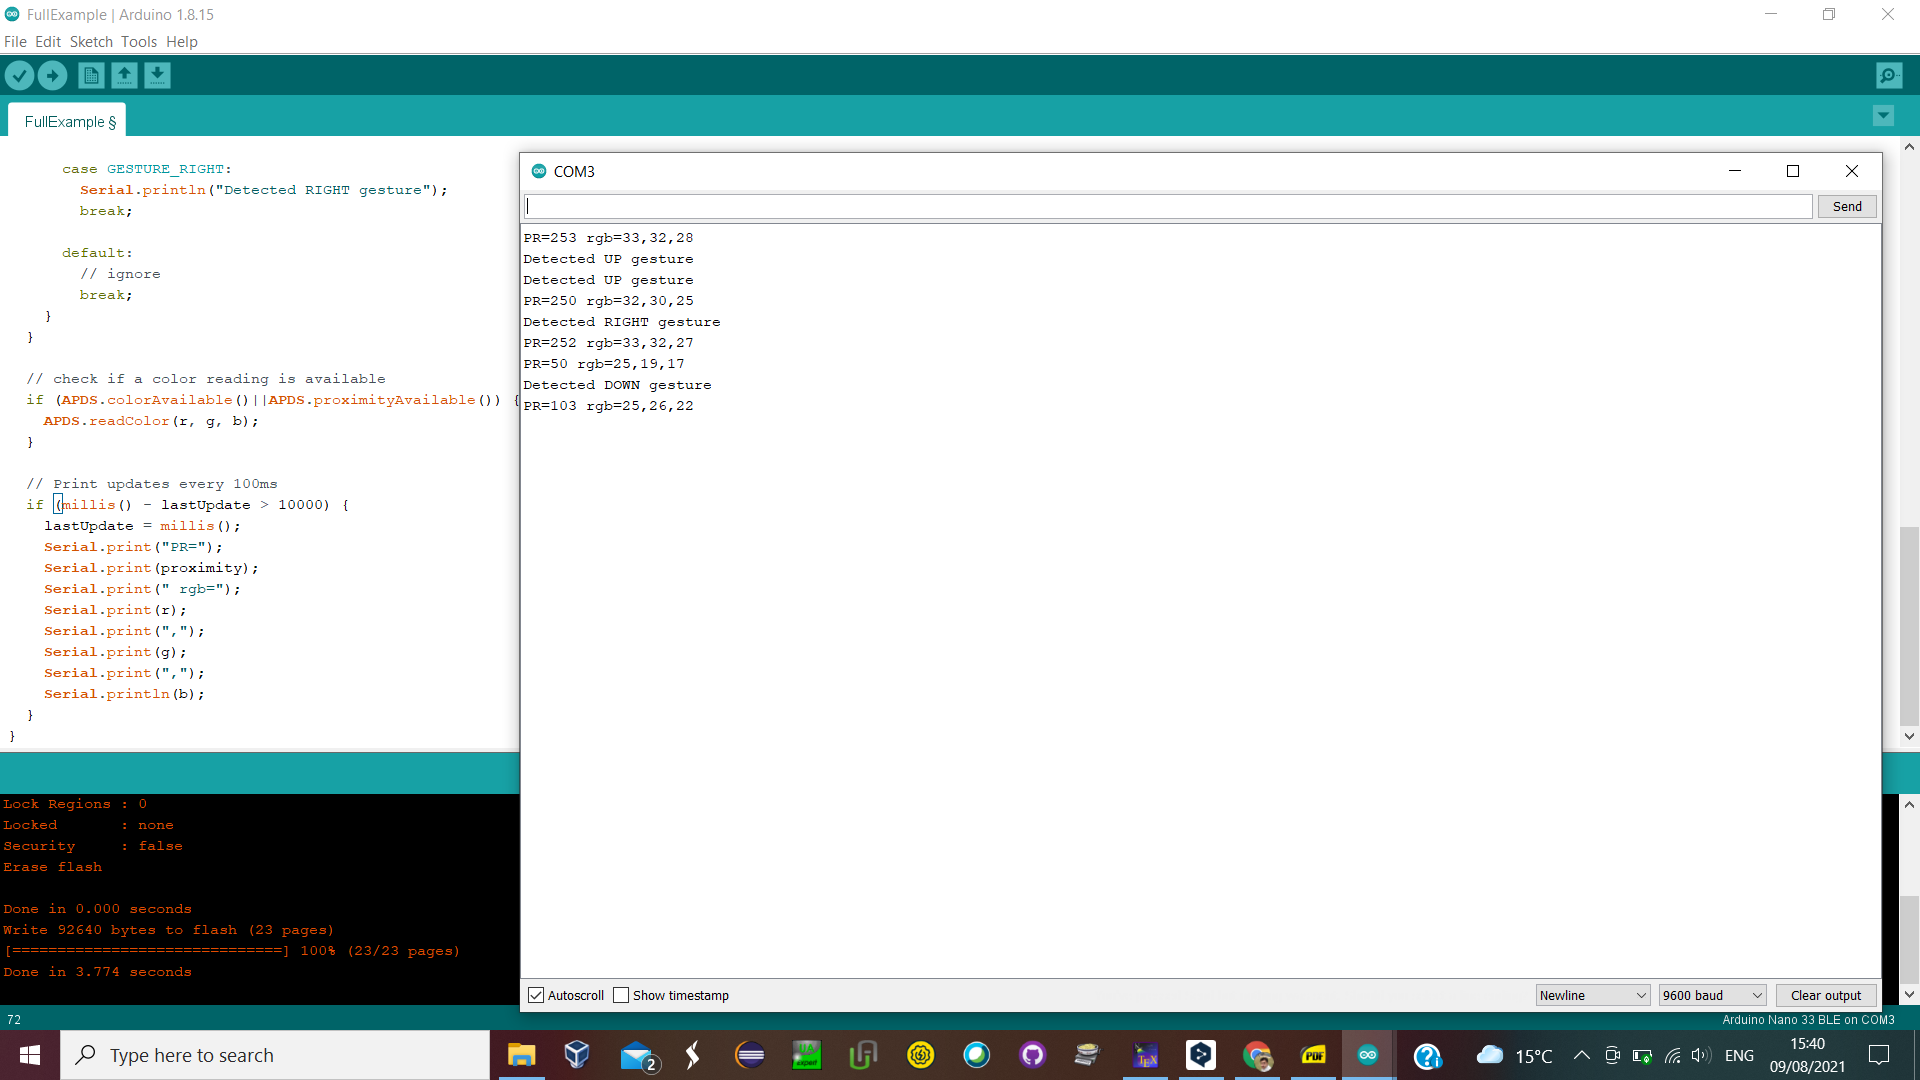
\includegraphics[width=9.5cm]{Nano33BLESense/APDS-Output}
    \captionof{figure}{Gesture, Proximity, Color Sensor Output Window}
    \label{fig:2}
\end{center}

We can also run the single funcnality of this sensor too, e.g; if we just need to capture the color of product, we can also run the color detection program. It depends upon the application and we can implement our application and modify the code as per our desire results.


{
    \captionof{code}{Simple sketch using the sensor APDS9960}\label{TestAPDS9960}
    \ArduinoExternal{}{../../Code/Nano33BLESense/Test/TestAPDS9960.ino}
}




%%%%%%%%%%%%%%%%%%%%%%%%%%%%%%%%%%



\section{Further Readings}




 










